% Section 4: Laboratory experiment. Facts: ldv_processing_log.md items 0-2, step 1; figures F4, A1, A2.
\section{Laboratory experiment}\label{sec:experiment}
\begin{notes}
\item Specimen: PMMA plate $900\times835\times10$\,mm on foam pads; four PZT blocks $10\times10\times7$\,mm (5.3\,g) bonded on the back face; defects drilled from the back after the pristine scan: D1, D2 blind holes \O10\,mm, 6\,mm deep; D3 through-hole \O10\,mm; D4 blind hole \O8\,mm, 6\,mm deep; M1 steel cube 10\,mm glued on the back (F4, drawing A1).
\item Excitation: Ricker 40\,kHz; main mode A0 ($\lambda\approx25$\,mm, phase velocity $\approx1000$\,m/s); S0 visible at about 10\,\% of A0.
\item LDV: Polytec 3-D PSV on a robot (A2); $v_z$ used; fs 3.125\,MHz, 1.6\,ms, 20 averages, about 3.8\,s per point and shot.
\item Scans: pristine (6\,mm grid, 1650 points) and defect scan (3\,mm grid, 6418 points, about 7\,h per shot). The plate moved between the scans (registration on the direct waves: $T=(-3.6,-2.7)$\,mm), so the defect scan is inverted directly, without pristine subtraction.
\item Shots -- state neutrally: because of a fault in the excitation script, S1 is driven in every acquisition; the four shots are S1, S1+S2, S1+S3, S1+S4. The model simulates exactly the driven transducers of each shot. Two-shot set: S1 and S1+S3 (chosen as the farthest pair, without using the defects); one-shot set: S1+S3 only.
\item Pristine scan also had wrong-source points (independent clocks); the defect scan has none (timing fixed). Mention only as far as needed for the calibration (Sec.~\ref{sec:model}).
\item Preprocessing: band-pass 15--90\,kHz, resample 625\,kHz, window 400--1500\,\textmu s; dropouts (noise $>3\times$ median, about 10\,\%).
\item Every result-producing step is blind to the defects; their positions are used only for scoring.
\end{notes}
\begin{figure}[ht]\centering
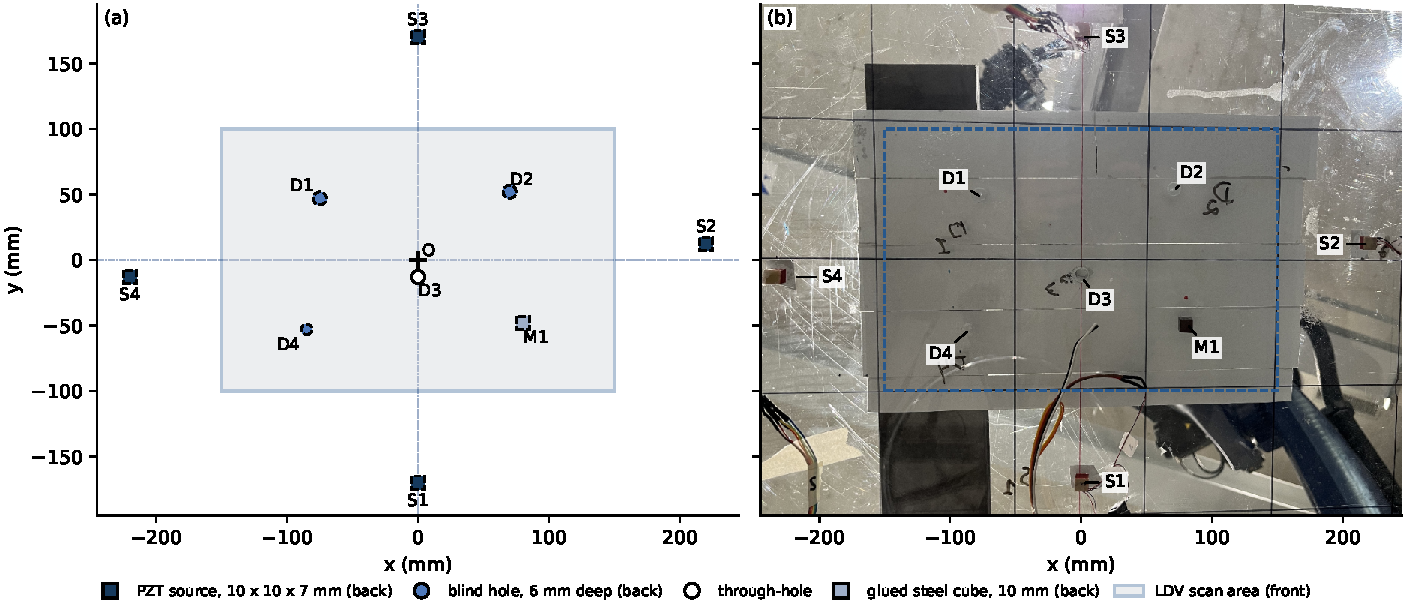
\includegraphics[width=\linewidth]{F4_specimen.pdf}
\caption{\textbf{Specimen.} (a) Front face (LDV side), positions from the scan centre O; (b) photo of the plate, top-down through the transparent PMMA, resampled into the same frame (homography on 9 control points, residuals $\le 2$\,mm) and annotated. Specimen: 10\,mm PMMA plate (900$\times$835\,mm), four PZT sources (10$\times$10$\times$7\,mm blocks, back face), blind holes D1, D2 (10\,mm) and D4 (8\,mm) 6\,mm deep from the back, through-hole D3 (10\,mm), glued steel cube M1 (10\,mm, back); dashed outlines = back face. Full drawing in Appendix Fig.~A1, laboratory setup in Fig.~A2.}\label{fig:specimen}
\end{figure}

